\chapter{Model Validation and Selection}

Choosing different exponential for the Hypothesis $H^0$ or $H^3$ we are changing the different shape of our function and every bigger polynomial contain the smaller one.
The question is, it is better to work with a smaller exponent or a bigger one? We can measure that with the sum of the error of all the point that we have, and in that case we can say that bigger polynomial can lower the \textbf{training} error made in the training set. In general at some degree our error can became equal to 0, but in that case we made an error called \textbf{overfitting}.
We can't specialized so much on our training data because the other data aren't as the training so small train error \textbf{does not guarantee good performance} outside the training set.
It is important to create another subset of data called \textbf{validation set}, the purpose of this subset is to probe the hypothesis we did in the training set with other data to see the performance.
The real importance is to divide the data we use to take the hypothesis and the  one to probe that the hypothesis work.

\begin{figure}[H]
    \centering
    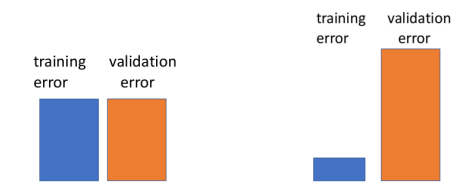
\includegraphics[scale=0.4]{images/MVS/MVS1.png}
    \caption{Example of validation error}
    \label{fig:enter-label}
\end{figure}

The aim is to reach the perfect balance without underfitting or overfitting so the lowest point on the training error and validation error to reach the correct number of complexity.
\begin{figure}[H]
    \centering
    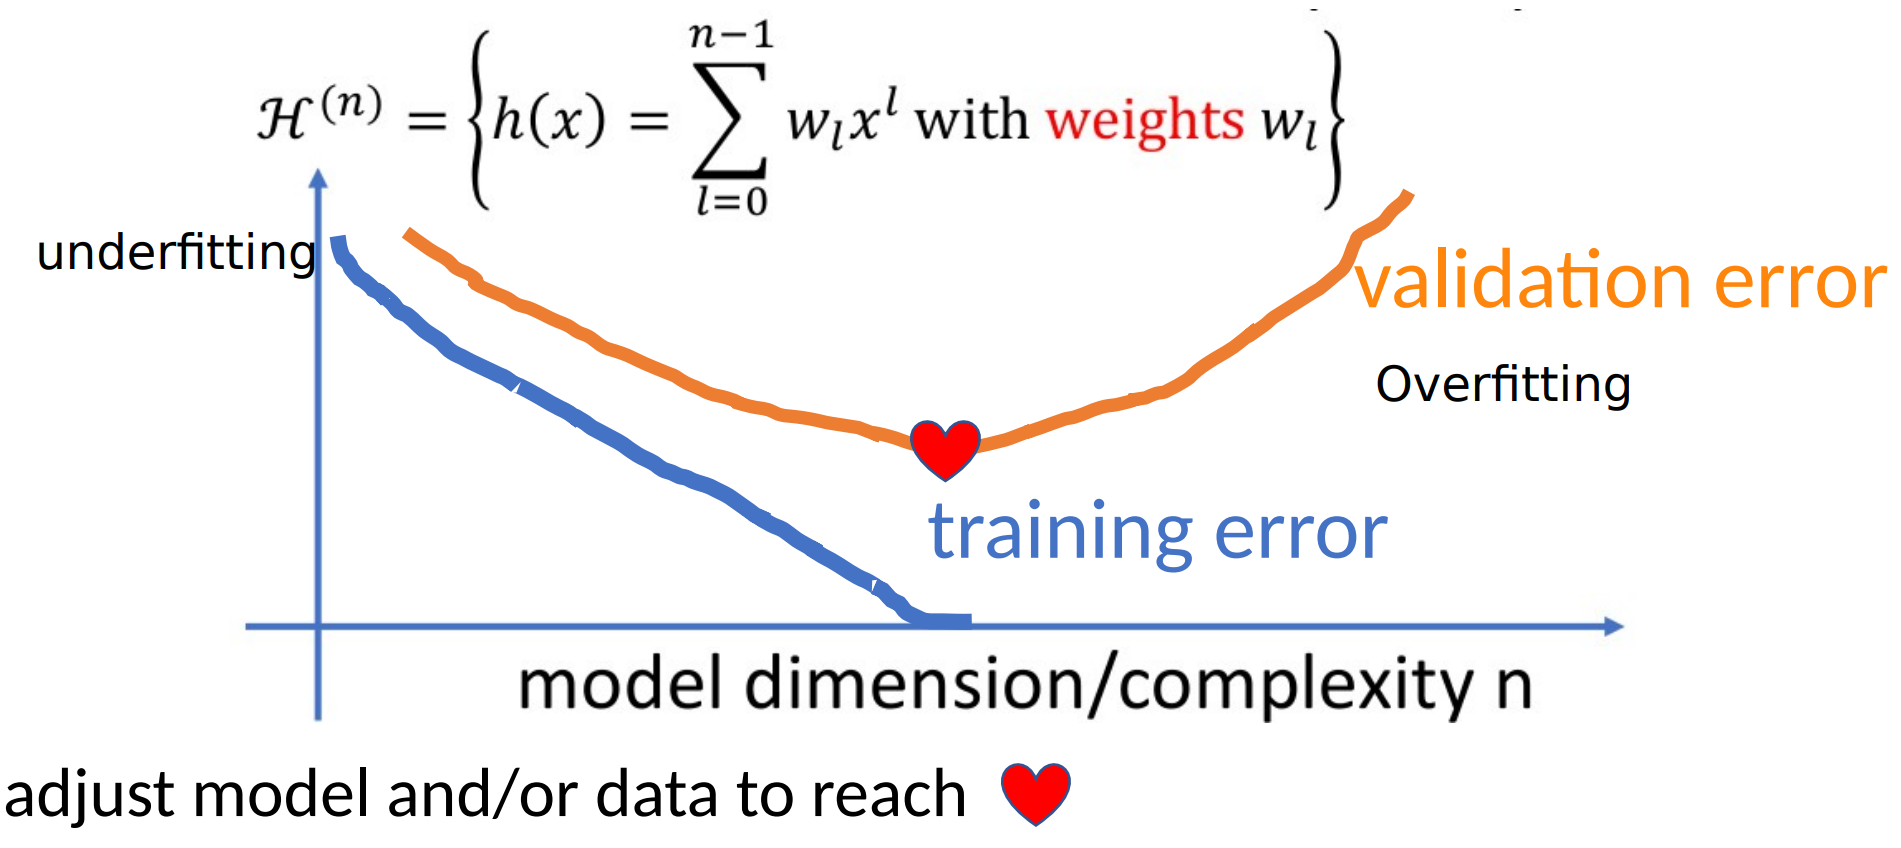
\includegraphics[scale=0.25]{images/MVS/MVS2.png}
    \caption{Train/Val Error vs. Model Complexity}
    \label{fig:enter-label}
\end{figure}

Another type of possible validation is the k-fold cross validation, the idea is to randomly split several times the data in different ways. The training error is the average empirical loss over the k training folds and the validation error is the average empirical loss over the k validation folds. Obviously the key is choose the number of folds because the train fold should be sufficiently large and the validation folds should be sufficiently large. there are also different type of k-fold like class-ratio preserving splitting, group-preserving splitting or temporal successive splitting

\begin{figure}[H]
    \centering
    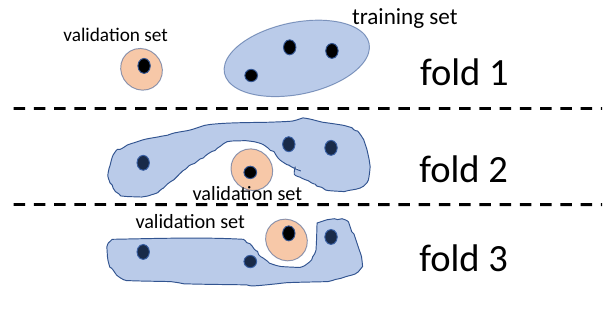
\includegraphics[scale=0.4]{images/MVS/MVS3.png}
    \caption{k-fold cross validation}
    \label{fig:enter-label}
\end{figure}

The test set is chosen model with validation error, Need a test set different from training and validation set.

The action to do are: 
\begin{itemize}
    \item input: list of candidate models
    \item  for each candidate model
        \begin{itemize}
            \item learn optimal hypothesis by minimize training error
            \item compute validation error on validation set
        \end{itemize}
    \item choose hypothesis with minimum validation error
    \item  compute test error of on test set
\end{itemize}